\documentclass{VUMIFInfBakalaurinis}
\usepackage{algorithmicx}
\usepackage{algorithm}
\usepackage{algpseudocode}
\usepackage{amsfonts}
\usepackage{amsmath}
\usepackage{bm}
\usepackage{caption}
\usepackage{color}
\usepackage{float}
\usepackage{graphicx}
% \usepackage{hyperref}  % Nuorodų aktyvavimas
\usepackage{listings}
\usepackage{subfig}
\usepackage{url}
\usepackage{wrapfig}

\usepackage{longtable}
\usepackage{rotating}

\definecolor{mygray}{rgb}{0.5,0.5,0.5}
\lstset{ %
  numbers=left,                    % where to put the line-numbers;
  numbersep=5pt,                   % how far the line-numbers are from the code
  numberstyle=\tiny\color{mygray}, % the style that is used for the line-numbers 
  breaklines=true                 % sets automatic line breaking
}



%%% Table of contents to list down to subsections and no further
\setcounter{tocdepth}{4}
 
%%% Number down to subsubsections only
\setcounter{secnumdepth}{4}

% Titulinio aprašas
\university{Vilniaus universitetas}
\faculty{Matematikos ir informatikos fakultetas}
\department{Programų sistemų katedra}
\papertype{Baigiamasis bakalauro darbas}
\title{Dalykinės srities modelio transformavimas į UML užduočių diagramas}
\titleineng{Deriving use cases from business process}
\status{4 kurso 1 grupės studentas}
\author{Aleksandras Sivkovas}
% \secondauthor{Vardonis Pavardonis}   % Pridėti antrą autorių
\supervisor{Prof. dr. Saulius Gudas}
\reviewer{prof. habil. dr. Vardaitis Pavardaitis}
\date{Vilnius \\ \the\year}

% Nustatymai
% \setmainfont{Palemonas}   % Pakeisti teksto šriftą į Palemonas (turi būti įdiegtas sistemoje)
\bibliography{bibliografija} 

\begin{document}
\maketitle

\tableofcontents

%Sutartinių ženklų, simbolių, vienetų ir terminų sutrumpinimų sąrašas (jeigu
%ženklų, simbolių, vienetų ir terminų bendras skaičius didesnis nei 10 ir
%kiekvienas iš jų tekste kartojasi daugiau nei 3 kartus).
\sectionnonum{Sąvokų apibrėžimai}
Šiame darbe naudojami žymėjimai:
\begin{enumerate}
	\item \textbf{BPMN} – modeliavimo kalba, skirta pavaizduoti informaciją plačiai auditorijai. \textbf{BPMN} buvo sukurta ir dažniausia naudojama pavaizduoti verslo procesams \cite{bpmnFormal}.
	\item \textbf{UML} – modeliavimo kalba, skirta suteikti standartinį sistemos analizės, architektūros, veikimo ir kūrimo pavaizdavimą \cite{omgUmlFormal}.
	\item \textbf{Sekų diagrama} – \textbf{UML} diagrama, skirta pavaizduoti žinučių tarp apibrėžtų objektų sekai tų objektų gyvavimo metu \cite{omgUmlFormal}.
	\item \textbf{Užduočių diagrama} – \textbf{UML} diagrama, skirta pavaizduoti pavaizduoti kaip gali būti naudojama programų sistema \cite{algUseCasesFromBpmn}.
\end{enumerate}


%Įvade apibūdinamas darbo tikslas, temos aktualumas ir siekiami rezultatai.
\sectionnonum{Įvadas}
Darbo tikslas – apibrėžti ir įgyvendinti algoritmą \textbf{BPMN} modelio transformacijai į \textbf{užduočių diagramas}.

Reikalavimų inžinerija yra sudėtinga programų kūrimo dalis. Proceso sudėtingumas dažnai tampa klaidų priežastimi. Čia atsiradusios klaidos sunkiai aptinkamos ir sukelia brangiai kainuojančias pasekmes, nes sekančiuose etapuose bus kuriama neteisingai apibrėžta programa. Norint išvengti klaidų galima kai kurias proceso veiklas automatizuoti.

Darbe bus tiriama verslo proceso transformacija į kuriamos programos \textbf{užduočių diagramas}. \textbf{Užduočių diagramos} yra svarbi reikalavimų inžinerijos dalis, kadangi ji apibrėžia kaip sistema bus naudojama. Įmonės dažniausiai žino kaip ir kokias veiklas jos vykdo. Verslo procesą galima apibrėžti \textbf{BPMN} diagramomis. Bet ne viską, kas yra \textbf{BPMN} modelyje, galima perkelti į \textbf{sekų diagramą}, todėl darbe bus apibrėžtas modifikuotas \textbf{BPMN} modelis, kuriame bus vaizduojama tik algoritmui aktuali informacija. Taip pat gali tekti pridėti papildomų atributų, kurie padės pasiekti tikslesnius rezultatus. Čia bus tiriama \textbf{BPMN} modelio transformacijos į \textbf{sekų diagramas} algoritmas.

Siekiami rezultatai yra:
\begin{enumerate}
	\item Modifikuoto \textbf{BPMN} modelio apibrėžimas.
	\item Algoritmas galintis transformuoti \textbf{BPMN} modelį į \textbf{užduočių diagramą}.
	\item Programa demonstruojanti algoritmo veikimą.
\end{enumerate}


%Pagrindinėje tiriamojoje dalyje aptariama ir pagrindžiama tyrimo metodika;
%pagal atitinkamas darbo dalis, nuosekliai, panaudojant lyginamosios analizės,
%klasifikacijos, sisteminimo metodus bei apibendrinimus, dėstoma sukaupta ir
%išanalizuota medžiaga. 
\section{Algoritmas kurti \textbf{sekų diagramas} pagal \textbf{BPMN} pateiktą informaciją}
Šio darbo tikslas yra algoritmas atlikti diagramų transformacijai. Pirmiausia pateikiama tai, kas literatūroje rašoma apie \textbf{UML} diagramų transformavimo algoritmus. Vėliau sukuriamas siekiamas algoritmas.
\subsection{\textbf{UML} diagramų transformavimo algoritmai}
\subsubsection{\textbf{Užduočių diagramos} išvedimas iš \textbf{BPMN} modelio} \label{section:use_cases_from_bpmn}
Literatųroje yra parašyta apie \textbf{vartojimo atvejų diagramos} išvedimą iš \textbf{BPMN} modelio \cite{algUseCasesFromBpmn}. Darbe nagrinėjamas \cite{algUseCasesFromBpmn} straipsnyje aprašytas algoritmas (\ref{eq:use_cases_from_bpmn}). Imamas modifikuotas \textbf{BPMN} modelis (\ref{eq:use_cases_from_bpmn:bpmn_elements}) ir tie \textbf{vartojimo atvejų diagramos} komponentai, kurie gali būti iš jo išvesti (\ref{eq:use_cases_from_bpmn:use_case_elements}). 
\begin{align}
&BPMNElements = \left\{Start,End,Role,Branch,Task,Transition\right\}; \label{eq:use_cases_from_bpmn:bpmn_elements} \\
\begin{split}
&UseCasesElements = \left\{Actor, Generalization, Association,Use Case,\right. \\
&\left. Include, Extension Point, Extend\right\}; \label{eq:use_cases_from_bpmn:use_case_elements}\\
\end{split} \\
&BPMN(BPMNModelElements) \Rightarrow UseCases(UseCasesElements); \label{eq:use_cases_from_bpmn}
\end{align}

Algoritmo autoriai pirmiausia siūlo surasti ryšius tarp modelių. juostos atitinka aktorius. Užduotys tuo tarpu grupuojamos, kol nepasiekia maksimalaus skaičiaus vykdomų be pertraukos, tos pačios juostos ir pagaminančių rezultatą. Tokia grupė pavadinama žingsniu ir yra laikoma atitinkančia vartojimo atvejį. Taip  išsiaiškinami transformacijos žingsniai. Tuomet lieka tik formaliai užrašyti kaip jie gali būti vykdomi ir surasti kaip dar galima būtų panaudoti informaciją, patikslinti ir suprastinti gautoms diagramoms.

Algoritmas Pirmiausia sudėlioja pavienes užduotis į proceso žingsnius. Vėliau juostos tampa aktoriais, o žingsniai jose – vartojimo atvejais. Galiausiai pasikartojančios užduotis išimamos iš žingsnių ir prijungiamos asociacija įtraukia arba išplečia pagal situaciją.


\subsection{\textbf{Užduočių diagramos} išvedimas iš \textbf{BPMN} modelio}

Šio darbo tikslas, algoritmas galintis gauti \textbf{užduočių diagramoms} iš \textbf{BPMN} modelio, bus kuriamas pagal \ref{section:use_cases_from_bpmn} aprašytą algoritmo sukūrimo pavyzdį. Pirmiausia bus rasti ryšiai tarp diagramų, vėliau sukurtas būdas juos panaudoti, galiausiai panaudota likusi modelio informacija patikslinti ir suprastinti diagramoms.

\subsubsection{Ryšiai tarp \textbf{BPMN} ir \textbf{sekų diagramų}} \label{section:relations_sd_bpmn}

Norint duomenis iš vieno modelio perkelti į kitą galima pasinaudoti ryšiais esančiais tarp jų.

\begin{center}
    \begin{longtable}{ | c | c |  c | c | c | c |}
    \caption{Ryšiai tarp \textbf{BPMN} ir \textbf{sekų diagramų}}
	\label{tab:relations_sd_bpmn}
    \\ \hline 
     & 
     %\begin{turn}{-90}
     Aktorius 
     %\end{turn} 
     & 
     %\begin{turn}{-90}
     Vartojimo atvejis 
     %\end{turn}  
     & 
     %\begin{turn}{-90}
     Asociacija 
     %\end{turn}  
     & 
     %\begin{turn}{-90}
     Įtraukia 
     %\end{turn} 
     & 
     %\begin{turn}{-90}
     Išplečia 
     %\end{turn} 
     \\ 
    \hline 
    Juosta & + & & + & + & + \\
    \hline
    Įvykis  & & & & & \\
    \hline 
    Veikla  & & + & + & + & + \\
    \hline 
    Sekos srautas  & & + & & & \\
    \hline
    Duomenų objektas  & & & & & \\
    \hline
    Pranešimų srautas  & & & & & \\
    \hline
    Sprendimas  & & & & & \\
    \hline
    \end{longtable}
\end{center} 

\begin{enumerate}
	\item Aktorius – galima gauti iš informacijos esančios juostoje. 
	\item Vartojimo atvejis – gaunamas iš informacijos veiklose.
	\item Asociacija – ryšys tarp juostos ir veiklų joje.
	\item Įtraukia – pasikartojančios veiklos.
	\item Išplečia – ryšys randamas kai veikla yra atskiras kitos veiklos atvejis.
\end{enumerate} 

Rasti ryšiai taip pat parodo kurie komponentai bus imami ir kurie gaunami. Taigi galima apibrėžti \textbf{BPMN} ir \textbf{Užduočių diagramas}. Tai taps algoritmo įvestimi ir išvestimi.

%Citavimo pavyzdžiai: cituojamas vienas šaltinis \cite{PvzStraipsnLt}; cituojami
%keli šaltiniai \cite{PvzStraipsnEn, PvzKonfLt, PvzKonfEn, PvzKnygLt, PvzKnygEn,
%PvzElPubLt, PvzElPubEn, PvzMagistrLt, PvzPhdEn}.
\subsubsection{BPMN diagrama}
\textbf{BPMN} specifikacija leidžia atvaizduoti gana nemažai verslo proceso atributų \cite{bpmnFormal}. Bet šiame darbe ji bus nagrinėjama tik kaip įvesties duomenų formatas, naudojamas apibrėžti informaciją pagal kurią bus kuriama \textbf{sekų diagrama}. Taigi daugelį \textbf{BPMN} komponentų galima tiesiog ignoruoti, nes jie neturi jokios įtakos algoritmo vykdymo rezultatui. Norint pabrėžti svarbią informaciją, darbe bus tiriamos tik tos \textbf{BPMN} savybės kurios gali įtakoti algoritmo vykdymo rezultatą. Atitinkami komponentai pavaizduoti \ref{tab:investigated_bpmn_components} lentelėje.
\newcounter{counter:table:reset}
\newcounter{counter:table}[counter:table:reset]
\newcommand\rownumber{\stepcounter{counter:table}\arabic{counter:table}}
\begin{center}
    \begin{longtable}{ | p{0.5cm} | p{2cm} |  p{7cm} | p{4cm} |}
    \caption{BPMN diagramos komponentai}
	\label{tab:investigated_bpmn_components}
    \\ \hline 
    Nr. & Komponentas & Aprašymas & Žymėjimo pavizdys\\ 
    \hline 
    \rownumber & Juosta & Komponentas žymintis diagramos dalyvį ir nurodantis, kad jis atsakingas už veiklų esančių šiame komponente vykdymą. & \vtop{\hbox{\strut }\hbox{\strut 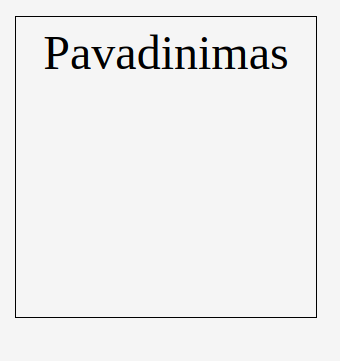
\includegraphics[width=3cm]{img/bpm-components/pool}}} \\
    \hline
     \rownumber & Įvykis & Komponentas žymintis, kad ivyko kažkas kas įtakojo proceso būseną. & \vtop{\hbox{\strut }\hbox{\strut 
\includegraphics[width=3cm]{img/bpm-components/event}}} \\ 
    \hline 
    \rownumber & Veikla & Komponentas žymintis užduoties vykdymo procesą & \vtop{\hbox{\strut }\hbox{\strut 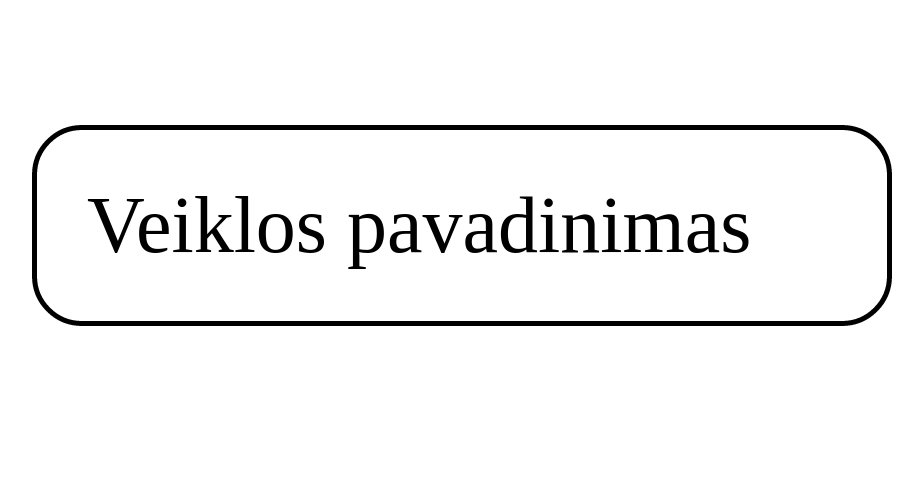
\includegraphics[width=3cm]{img/bpm-components/activity}}}\\
    \hline 
    \rownumber & Sekos srautas & Komponentas žymintis veiklų seką. & \vtop{\hbox{\strut }\hbox{\strut 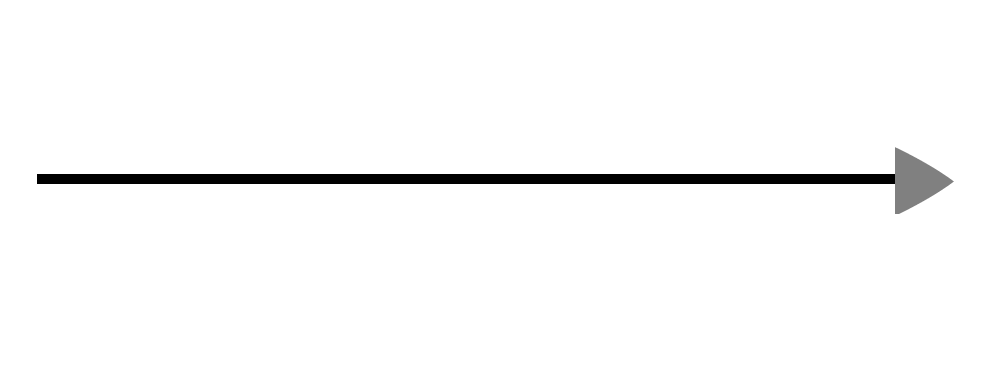
\includegraphics[width=3cm]{img/bpm-components/transition}}}\\
    \hline
%    \rownumber & Duomenų objektas & Komponentas žymintis sukuriamus arba įeities duomenis. & \vtop{\hbox{\strut }\hbox{\strut 
\includegraphics[width=3cm]{img/bpm-components/data_object}}}\\
%    \hline
%    \rownumber & Pranešimų srautas & Komponentas žymintis duomenų apsikeitimo srautus. & \vtop{\hbox{\strut }\hbox{\strut 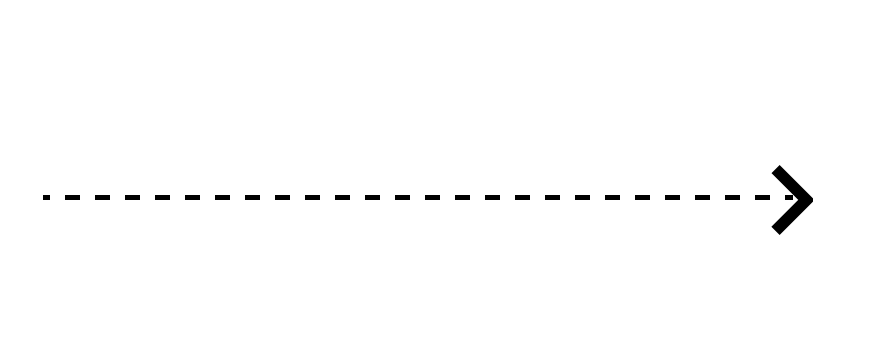
\includegraphics[width=3cm]{img/bpm-components/message_flow}}}\\
%    \hline
    \rownumber & Sprendimas & Komponentas žymintis sekos srautų išsišakojimą. & \vtop{\hbox{\strut }\hbox{\strut 
\includegraphics[width=3cm]{img/bpm-components/gateway}}}\\
    \hline
    \end{longtable}
\end{center}

Darbe bus nagrinėjamas procesas kuriam kuriama programų sistema, todėl materialios  veiklos bus atskirtos nuo duomenų tvarkymo veiklų \cite{bpmnPorterModel}. \textbf{BPMN} diagrama bus vaizduojama kaip detalizuotas M. Porterio vertės grandinės modelis (\ref{img:detalized_porter_vcm} pav), todėl į apibrėžimą įtrauktas sprendimas, kuris bus naudojamas išsišakojimui pavaizduoti. Tokiu būdu dėmesys telkiamas ties informacijos procesais.

\begin{figure}[H]
	\centering
	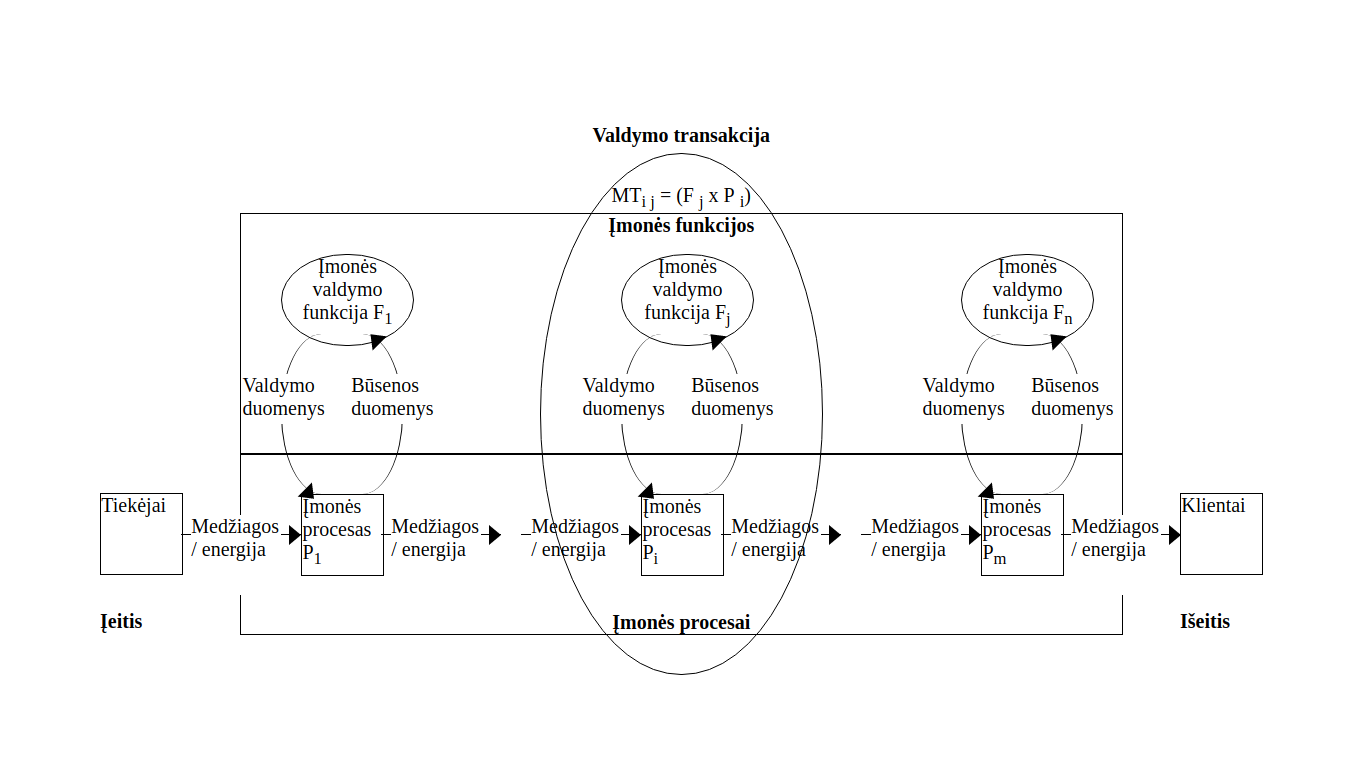
\includegraphics[width=\textwidth]{img/detalized_porter_vcm}
	\caption{Detalizuotas M. Porterio vertės grandinės modelis}
	\label{img:detalized_porter_vcm}
\end{figure} 

\subsubsection{Užduočių diagrama}

Čia pateikiamas \textbf{užduočių diagramos} naudojamos darbe apibrėžimas. Tai bus algoritmo rezultato formatas. Siekiama gauti kiek įmanoma tikslesnę užduočių diagramą. Jos komponentai pateikiam \ref{tab:investigated_use_case_diagram_components} lentelėje.
\stepcounter{counter:table:reset}
\begin{center}
    \begin{longtable}{ | p{0.5cm} | p{2cm} |  p{7cm} | c |}
    \caption{\textbf{Užduočių diagramos} komponentai}
	\label{tab:investigated_use_case_diagram_components}
    \\ \hline 
    Nr. & Komponentas & Aprašymas & Žymėjimo pavizdys\\ 
    \hline 
    \rownumber & Aktorius & Komponentas žymintis sistemos naudotojo tipą. & \vtop{\hbox{\strut }\hbox{\strut 
\includegraphics[width=3cm]{img/use_case_components/actor}}} \\
    \hline
    \rownumber & Vartojimo atvejis & Komponentas specifikuojantis elgsenų aibę, kuri generuoja rezultatą. & \vtop{\hbox{\strut }\hbox{\strut 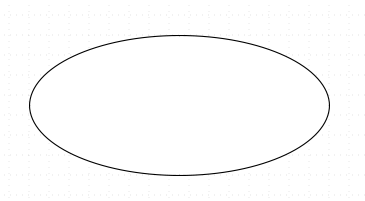
\includegraphics[height=3cm]{img/use_case_components/use_case}}} \\
    \hline
     \rownumber & Asociacija & Komponentas žymintis ryšį tarp aktoriaus ir vartojimo atvejo. & \vtop{\hbox{\strut }\hbox{\strut 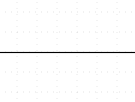
\includegraphics[width=3cm]{img/use_case_components/association}}} \\
    \hline
     \rownumber & Įtraukia & Komponentas žymintis elgseną kuri yra bendra keliems vartojimo atvejams, todėl ji parodoma atskirai nuo jų, kad būtų galima perpanaudoti. & \vtop{\hbox{\strut }\hbox{\strut 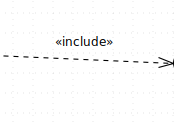
\includegraphics[width=3cm]{img/use_case_components/includes}}} \\
    \hline
    \rownumber & Išplečia & Komponentas žymintis, kad esant tam tikram atvejui vartojimo atvejis įtraukia papildomus vartojimo atvejus. & \vtop{\hbox{\strut }\hbox{\strut 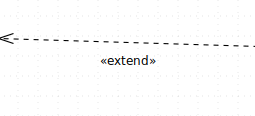
\includegraphics[width=3cm]{img/use_case_components/extend}}} \\
    \hline
    \end{longtable}
\end{center}

\subsubsection{Ryšių tarp diagramų panaudojimas transformacijai}

Rasti ryšiai parodo į kokius \textbf{BPMN} komponentus reikia žiūrėti išvedant \textbf{užduočių diagramos} dalis. Toliau peržiūrimi diagramos variantai ir sudėliojami konkretūs žingsniai kuriuos reikia atlikti. Galiausiai gaunamas pseudokodas (Listing \ref{lst:bpmn_to_sd_algorythm_pseudocode}). 

%\begin{lstlisting}[language=java, caption={\textbf{UML} \textbf{Sekų diagramos} gavimo iš \textbf{BPMN} modelio algoritmo pseudokodas}, label={lst:bpmn_to_sd_algorythm_pseudocode}]
%\end{lstlisting}
\lstinputlisting[language=java, caption={\textbf{UML} \textbf{Sekų diagramos} gavimo iš \textbf{BPMN} modelio algoritmo pseudokodas}, label={lst:bpmn_to_sd_algorythm_pseudocode}]{algorythm-pseudocode/useCasesFromBPMN}

\begin{enumerate}
	\item Pirmiausia imamas transakcijos procesas. 
	\item Vėliau jam sukuriami vartojimo atvejai funkcija getUseCasesForProcess (Listing  \ref{lst:bpmn_to_sd_algorythm_pseudocode_getUseCasesForProcess}).
	\lstinputlisting[language=java, caption={Funkcija getUseCasesForProcess}, label={lst:bpmn_to_sd_algorythm_pseudocode_getUseCasesForProcess}]{algorythm-pseudocode/getUseCasesForProcess}
	Joje funkcija addCycledFlows (Listing  \ref{lst:bpmn_to_sd_algorythm_pseudocode_addCycledFlows}) paima tik tuos sekos srautus, kurie sudaro ciklą su procesu.
	\lstinputlisting[language=java, caption={Funkcija addCycledFlows}, label={lst:bpmn_to_sd_algorythm_pseudocode_addCycledFlows}]{algorythm-pseudocode/addCycledFlows}
	
	\item Sukurti vartojimo atvejai pridedami prie jau gautų vartojimo atvejų kartu su ryšiais tarp jų funkcija addNewUsecases (Listing  \ref{lst:bpmn_to_sd_algorythm_pseudocode_addNewUsecases}). 
\lstinputlisting[language=java, caption={Funkcija addNewUsecases}, label={lst:bpmn_to_sd_algorythm_pseudocode_addNewUsecases}]{algorythm-pseudocode/addNewUsecases}	

	\item Vėliau gaunamos visos diagramos funkcijos (Listing  \ref{lst:bpmn_to_sd_algorythm_pseudocode_getFunctions}).
	\lstinputlisting[language=java, caption={Funkcija getFunctions}, label={lst:bpmn_to_sd_algorythm_pseudocode_getFunctions}]{algorythm-pseudocode/getFunctions}
	\item Randamos bendros funkcijos tarp tranzakcijų ir sukuriami apibendrinantys vartojimo atvejai (Listing  \ref{lst:bpmn_to_sd_algorythm_pseudocode_addGeneralUseCases}).
	\lstinputlisting[language=java, caption={Funkcija addGeneralUseCases}, label={lst:bpmn_to_sd_algorythm_pseudocode_addGeneralUseCases}]{algorythm-pseudocode/addGeneralUseCases}
	\item Galiausiai randamos nepanaudotos funkcijos ir sukuriami vartojimo atvejai su perspėjimais \ref{lst:bpmn_to_sd_algorythm_pseudocode_addUnusedCases}).
	\lstinputlisting[language=java, caption={Funkcija addUnusedCases}, label={lst:bpmn_to_sd_algorythm_pseudocode_addUnusedCases}]{algorythm-pseudocode/addUnusedCases}
\end{enumerate} 


%Iš diagramos \ref{img:bpmn} gaunama diagrama \ref{img:sequence}.

%\begin{figure}[H]
%	\centering
%	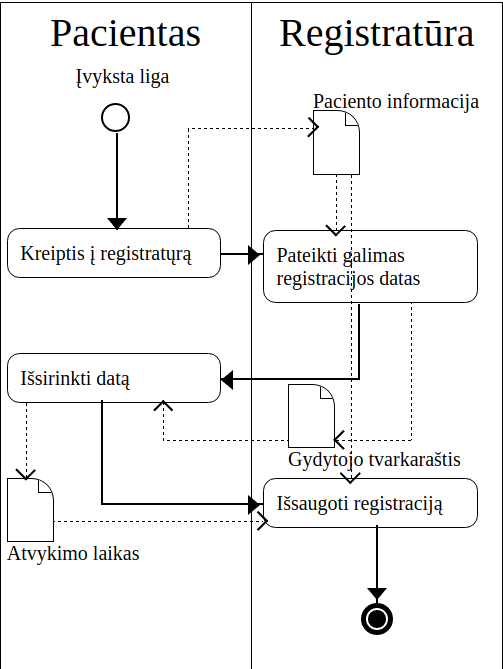
\includegraphics[scale=0.5]{img/bpmn_diagrama}
%	\caption{\textbf{BPMN} diagrama}
%	\label{img:bpmn}
%\end{figure} 
%\begin{figure}[H]
%	\centering
%	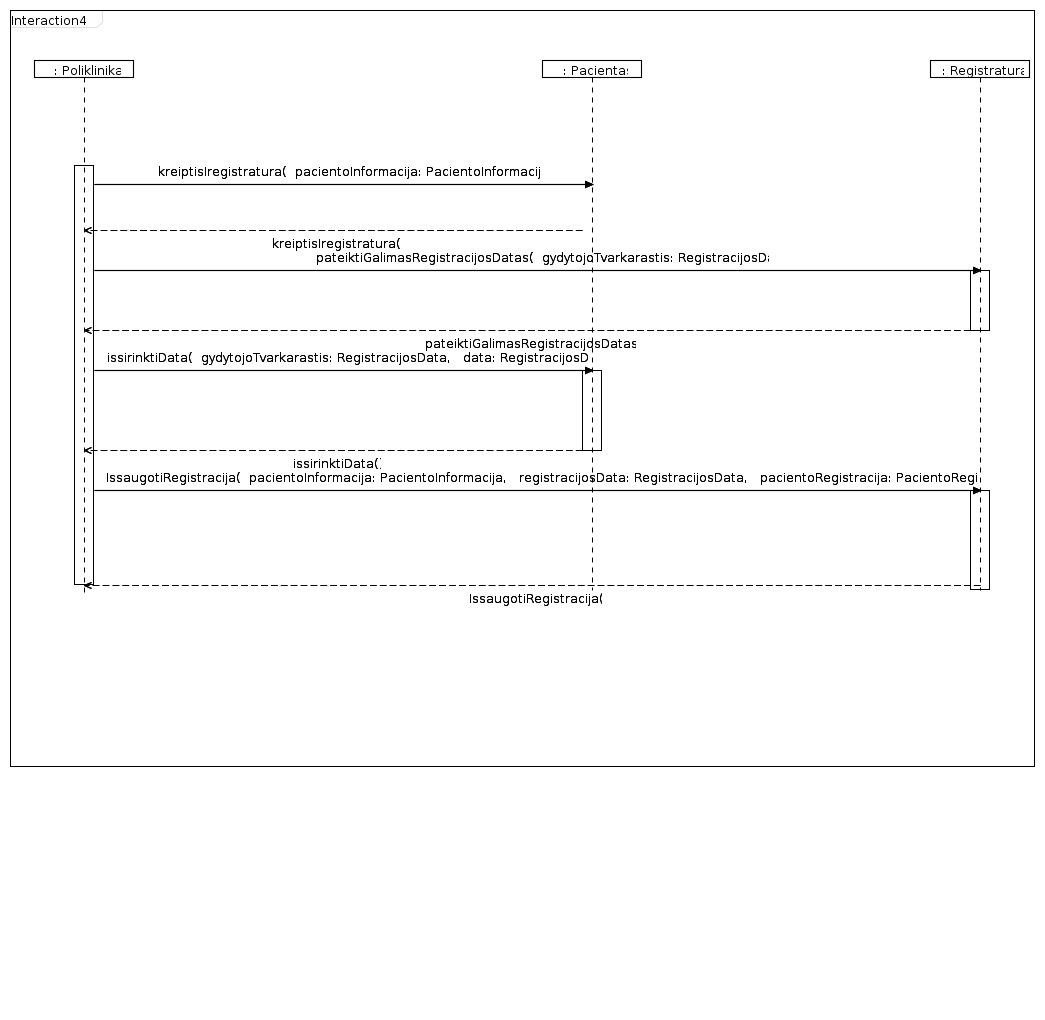
\includegraphics[scale=0.5]{img/sequence_example}
%	\caption{\textbf{sekų diagramą} diagrama}
%	\label{img:sequence}
%\end{figure} 

\subsubsection{Likusios informacijos panaudojimas suprastinti ar patikslinti diagramai}


\section{Programa \textbf{BPMN} transformacijai į \textbf{sekų diagramą}}   


%Išvadose ir pasiūlymuose, nekartojant atskirų dalių apibendrinimų,
%suformuluojamos svarbiausios darbo išvados, rekomendacijos bei pasiūlymai.
\sectionnonum{Išvados}

%Šiame skyriuje pateikiamos išvados (reziume) anglų kalba.
\sectionnonum{Conclusions}


% bibliografija.bib faile. Šaltinių sąraše nurodoma panaudota literatūra,
% kitokie šaltiniai. Abėcėlės tvarka išdėstoma tik darbe panaudotų (cituotų,
% perfrazuotų ar bent paminėtų) mokslo leidinių, kitokių publikacijų
% bibliografiniai aprašai (šiuo punktu pasirūpina LaTeX). Aprašai pateikiami
% netransliteruoti.
\printbibliography[heading=bibintoc] % Literatūros šaltiniai aprašomi


% Prieduose gali būti pateikiama pagalbinė, ypač darbo autoriaus savarankiškai
% parengta, medžiaga. Savarankiški priedai gali būti pateikiami kompiuterio
% diskelyje ar kompaktiniame diske. Priedai taip pat vadinami ir numeruojami.
% Tekstas su priedais siejamas nuorodomis (pvz.: \ref{img:mlp}).
\appendix  % Priedai


%\section{Niauroninio tinklo struktūra}
%\begin{figure}[H]
%    \centering
%    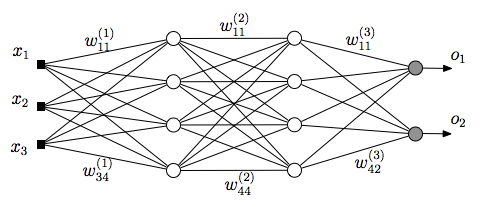
\includegraphics[scale=0.5]{img/MLP}
%    \caption{Paveikslėlio pavyzdys}
%    \label{img:mlp}
%\end{figure}


%\section{Eksperimentinio palyginimo rezultatai}
% tablesgenerator.com - converts calculators (e.g. excel) tables to LaTeX
%\begin{table}[H]\footnotesize
%  \centering
%  \caption{Lentelės pavyzdys}
%  {\begin{tabular}{|l|c|c|} \hline
%    Algoritmas & $\bar{x}$ & $\sigma^{2}$ \\
%    \hline
%    Algoritmas A  & 1.6335    & 0.5584       \\
%    Algoritmas B  & 1.7395    & 0.5647       \\
%    \hline
%  \end{tabular}}
%  \label{tab:table example}
%\end{table}

\end{document}
